\documentclass{standalone}
\usepackage{tikz}
\usepackage{ctex,siunitx}
\setCJKmainfont{Noto Serif CJK SC}
\usepackage{tkz-euclide}
\usepackage{amsmath}
\usepackage{wasysym}
\usetikzlibrary{patterns, calc}
\usetikzlibrary {decorations.pathmorphing, decorations.pathreplacing, decorations.shapes,}
\begin{document}
\small
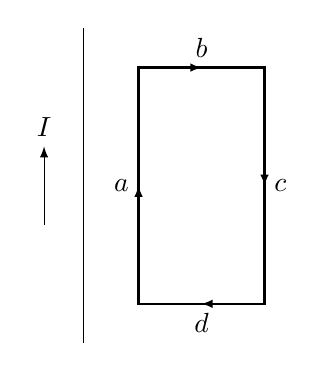
\begin{tikzpicture}[>=latex,scale=1]
  \draw (0,.5)--(0,4.5);
  \draw[->] (-.5,2)--(-.5,3)node [above]{$I$};
  \draw[thick] (1-.3,1) rectangle (2+.3,4);
  \draw[->] (1-.3,1.5)--(1-.3,2.5)node [left]{$a$};
  \draw [->](2+.3,3)--(2+.3,2.5)node [right]{$c$};
  \draw[->] (1-.3,4)--(1.5,4)node [above]{$b$};
  \draw [->](2+.3,1)--(1.5,1)node [below]{$d$};
\end{tikzpicture}
\end{document}